\chapter{FIR Matched Filter Implementation}

\section{Matched Filter Theory}
A matched filter is the optimal linear filter for detecting a known signal in 
textit{additive white Gaussian noise}. For a sampled BPSK reference pulse \(s_1[n]\), 
the FIR matched filter impulse response is the time-reversed version of the signal:
\[
h_{mf}[n]=s_1[N-1-n]
\]

This means the filter coefficients are simply the reversed samples of the reference BPSK waveform. 
When the received signal is passed through this filter, the output peaks at the sampling instant if the transmitted waveform matches the reference.

\section{Python Implementation}
The following Python code generates the matched filter coefficients and plots the impulse \\response.

\begin{lstlisting}[style=pythonstyle, caption={FIR Matched Filter Coefficients and Frequency \\Response}]
import numpy as np
import matplotlib.pyplot as plt

A = 1
fc = 15000
Rb = 1000
fs = 200000

Tb = 1 / Rb
t = np.arange(0, Tb, 1/fs)

s1 = A * np.cos(2 * np.pi * fc * t)
hmf = s1[::-1]

plt.figure(figsize=(10,4))
plt.stem(hmf, basefmt=" ")
plt.xlabel('Sample Index')
plt.ylabel('Amplitude')
plt.title('FIR Matched Filter Coefficients')
plt.grid(True)
plt.tight_layout()
plt.show()

w = np.linspace(0, np.pi, 1024)
H = np.fft.fft(hmf, 1024)

plt.figure(figsize=(10,4))
plt.plot(np.abs(H))
plt.xlabel('Frequency Index')
plt.ylabel('Magnitude')
plt.title('Frequency Response of FIR Matched Filter')
plt.grid(True)
plt.tight_layout()
plt.show()
\end{lstlisting}

\section{Discussion}
The FIR matched filter is stable because it has a finite number of coefficients. 
A finite impulse response system is always bounded-input bounded-output stable, 
which makes it practical for digital implementation.

The matched filter is equivalent to the correlator receiver because both perform the same \\mathematical operation: 
they measure the similarity between the received signal and a known reference waveform. 
The correlator computes an inner product directly, while the FIR matched filter produces the same result through convolution \
and sampling at the appropriate instant.

\section{Results and Discussion}
The matched filter coefficients are obtained by reversing the one-bit BPSK pulse. 
This gives the receiver a strong peak response at the correct sampling time, 
which improves detection in noise.

\begin{figure}[htbp]
    \centering
    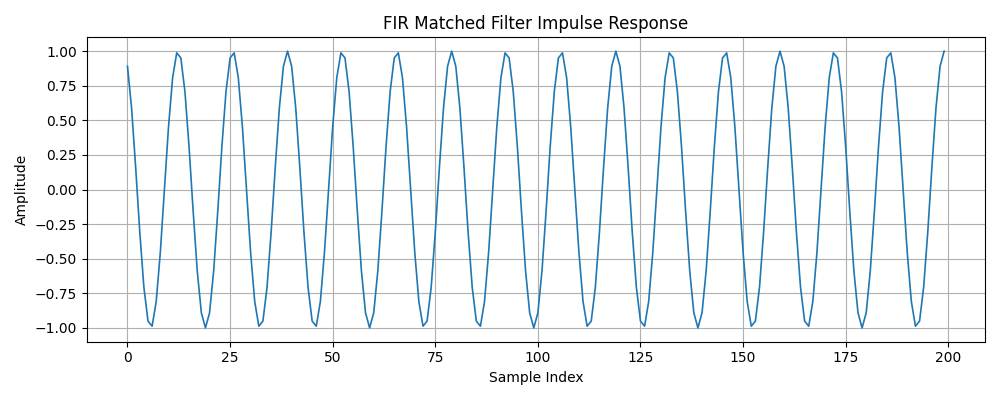
\includegraphics[width=0.8\textwidth]{plots/fir_impulse_response.png}
    \caption{FIR matched filter coefficients}
\end{figure}

\begin{figure}[htbp]
    \centering
    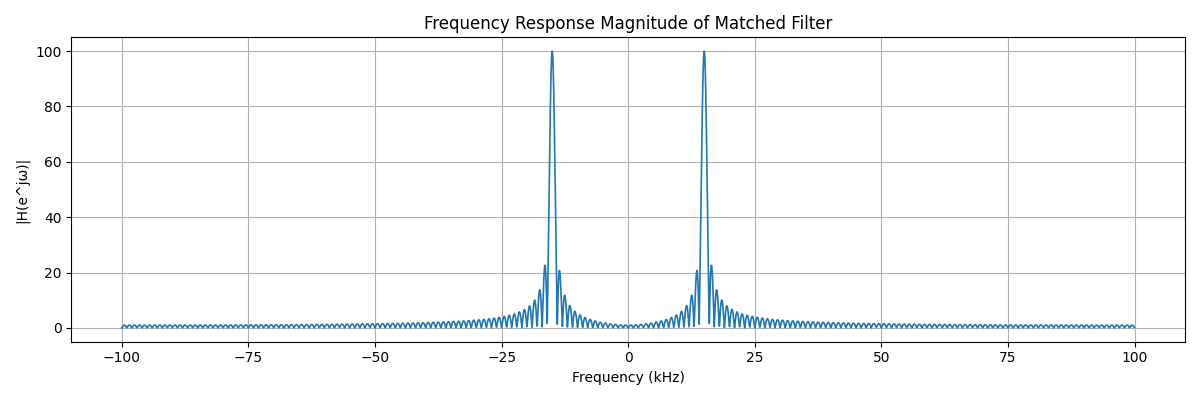
\includegraphics[width=0.8\textwidth]{plots/frequency_response_matched_filter.png}
    \caption{Frequency response of the FIR matched filter}
\end{figure}

In the final report, compare the decision output of the matched filter with the correlator receiver 
and mention that both give the same bit decisions when implemented correctly for the same reference pulse and 
sampling instant.